Figure 1 shows the uncalibrated spectral data for $^{241}$Am and $^{137}$Cs where the x axis is still
the channel number from the detector output.

\begin{figure}[H]
  \centering
  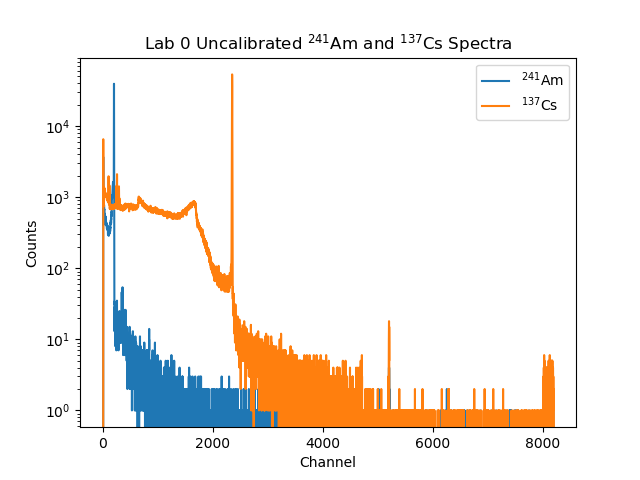
\includegraphics[width=0.6\textwidth]{am_cs_uncalibrated.png}
  \caption{Uncalibrated spectra for $^{241}$Am and $^{137}$Cs}
  \label{fig:uncalspectra}
\end{figure}


The next step is to take the accepted values for the full energy peaks for $^{241}$Am and $^{137}$Cs and preform
a linear calibration to fit the data to the proper energy.
\begin{center}
  \begin{equation}
    \label{eq:cal}
    y = mx+b
  \end{equation}
  where
  \begin{equation}
    \label{eq:slope}
    m = \frac{E_{Cs} - E_{Am}}{Ch_{Cs}-Ch_{Am}}
  \end{equation}
  and the intercept is found by
  \begin{equation}
    \label{eq:slope}
    b = -m*Ch_{Am} + E_{Am}
  \end{equation}
\end{center}
  Applying this fit yields our linear model:

\begin{figure}[H]
  \begin{center}
    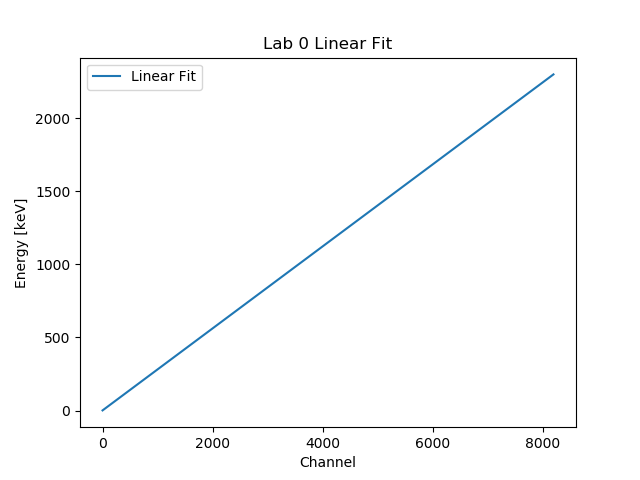
\includegraphics[width=10cm]{linear_fit.png}
    \caption{\label{fig:linfit}Linear Fit Model}
  \end{center}
\end{figure}


 When we apply this fit to the data and you can clearly see the 662 keV peak of $^{137}$Cs is properly calibrated.

 \begin{figure}[H]
   \begin{center}
     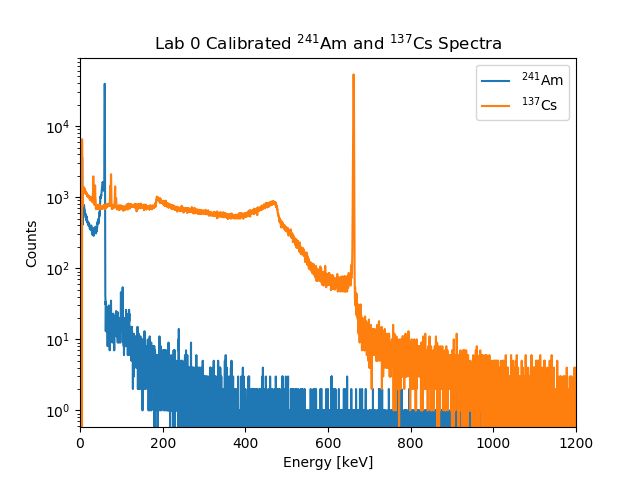
\includegraphics[width=10cm]{am_cs_calibrated.png}
     \caption{\label{fig:linfit}Calibrated Spectra for $^{241}$Am and $^{137}$Cs }
   \end{center}
 \end{figure}

 This model will then be applied to the $^{133}$Ba data, then compared to the accepted gamma energy values to
 evaluate the effectiveness of our calibration.
